\begin{enumerate}[label=\thechapter.\arabic*,ref=\thechapter.\theenumi]

\item Consider a unity-gain negative feedback system consisting of the plant $G\brak{s}$  and a proportional-integral controller. Let the proportional gain and integral
gain be 3 and 1, respectively. For a unit step reference input, the final values of the
controller output and the plant output, respectively, are
\begin{align}
    G\brak{s} = \frac{1}{\brak{s-1}} \notag
\end{align}\hfill (GATE EE 2023)\\
\solution 
\iffalse
\let\negmedspace\undefined
\let\negthickspace\undefined
\documentclass[journal,12pt,twocolumn]{IEEEtran}
\usepackage{cite}
\usepackage{amsmath,amssymb,amsfonts,amsthm}
\usepackage{algorithmic}
\usepackage{graphicx}
\usepackage{textcomp}
\usepackage{xcolor}
\usepackage{txfonts}
\usepackage{listings}
\usepackage{enumitem}
\usepackage{mathtools}
\usepackage{float}
\usepackage{gensymb}
\usepackage{comment}
\usepackage[breaklinks=true]{hyperref}
\usepackage{tkz-euclide} 
\usepackage{listings}
\usepackage{gvv}                                        
\def\inputGnumericTable{}                                 
\usepackage[latin1]{inputenc}                                
\usepackage{color}                                            
\usepackage{array}          
\usetikzlibrary{positioning, arrows.meta}
\usepackage{longtable}                                       
\usepackage{calc}                                             
\usepackage{multirow}                                         
\usepackage{hhline}                                           
\usepackage{ifthen}                                           
\usepackage{lscape}
\usepackage{amsmath}
\newtheorem{theorem}{Theorem}[section]
\newtheorem{problem}{Problem}
\newtheorem{proposition}{Proposition}[section]
\newtheorem{lemma}{Lemma}[section]
\newtheorem{corollary}[theorem]{Corollary}
\newtheorem{example}{Example}[section]
\newtheorem{definition}[problem]{Definition}
\newcommand{\BEQA}{\begin{eqnarray}}
\newcommand{\EEQA}{\end{eqnarray}}
\newcommand{\define}{\stackrel{\triangle}{=}}
\theoremstyle{remark}
\newtheorem{rem}{Remark}
\begin{document}

\bibliographystyle{IEEEtran}
\title{GATE-EE-Q14}
\author{EE23BTECH11015 - DHANUSH V NAYAK$^{*}$% <-this % stops a space
}
\maketitle
\newpage
\bigskip
\renewcommand{\thefigure}{\arabic{figure}}
\renewcommand{\thetable}{\theenumi}
\textbf{Question:}Consider a unity-gain negative feedback system consisting of the plant $G\brak{s}$  and a proportional-integral controller. Let the proportional gain and integral
gain be 3 and 1, respectively. For a unit step reference input, the final values of the
controller output and the plant output, respectively, are
\begin{align}
    G\brak{s} = \frac{1}{\brak{s-1}} \notag
\end{align} \hfill (GATE EE 2023)
\solution 
\fi
\begin{table}[H]
\centering
\renewcommand\thetable{1}
\setlength{\extrarowheight}{9pt}
\resizebox{0.5\textwidth}{!}{
\begin{tabular}{|c|c|c|}
\hline
\textbf{Parameter} & \textbf{Description} & \textbf{Value} \\ \hline
$K_{p}$ & Proportional Gain & 3  \\ \hline
$K_{i}$ & Integral Gain &1 \\ \hline
$r\brak{t}$& Reference Input & $u\brak{t}$ \\ \hline 
$w\brak{t}$& Controller Output & $?$ \\ \hline 
$y\brak{t}$ & Plant Output & $?$ \\ \hline
$e\brak{t}$ & Error Input & $r\brak{t}-y\brak{t}$ \\ \hline
\end{tabular}}
\caption{Parameter Table}
\label{tab:gate_ee_Q14}
\end{table}

From the\figref{fig:gate_ee_Q14_blockdiagram}:
\begin{align}
    E\brak{s}&= U\brak{s} - Y\brak{s}\label{eq:gate_ee_Q14.1}\\
W\brak{s} &= 3E\brak{s} + \frac{1}{s}E\brak{s}\label{eq:gate_ee_Q14.2}\\
    Y\brak{s} &= G\brak{s}W\brak{s} \label{eq:gate_ee_Q14.3}
\end{align}
Some results:
\begin{align}
    tx\brak{t} &\system{L} -\frac{d{X\brak{s}}}{ds} \label{eq:laplace_diff_prop}\\
    e^{-at}x\brak{t} &\system{L} X\brak{s+a}\label{eq:laplace_timeshifting_prop}
\end{align}
By using \eqref{eq:laplace_diff_prop} and \eqref{eq:laplace_timeshifting_prop}:
\begin{align}
    e^{-t}u\brak{t} &\system{L} \frac{1}{s+1} ,  Re\brak{s}>-1 \label{eq:gate_ee_Q14result.1}\\
    t e^{-t}u\brak{t} &\system{L} \frac{1}{\brak{s+1}^2},  Re\brak{s}>-1 
 \label{eq:gate_ee_Q14result.2}
\end{align}

\begin{figure}[H]
    \resizebox{0.9\textwidth}{!}{\tikzset{
    block/.style = {draw, fill=white, rectangle, minimum height=3em, minimum width=3em},
    tmp/.style  = {coordinate}, 
    minus/.style= {draw, fill=white, circle, node distance=1cm, append after command={\pgfextra \draw ($(\tikzlastnode.center) + (-0.15,0)$) -- ($(\tikzlastnode.center) + (0.15,0)$) node[above] {$-$}; \endpgfextra}},
    plus/.style= {draw, fill=white, circle, node distance=1cm, append after command={\pgfextra \draw ($(\tikzlastnode.center) + (-0.15,0)$) -- ($(\tikzlastnode.center) + (0.15,0)$) node[above] {$+$}; \endpgfextra}},
    input/.style = {coordinate},
    output/.style= {coordinate},
    pinstyle/.style = {pin edge={to-,thin,black}}
}


\begin{tikzpicture}[auto, node distance=2cm,>=latex]
    \node [input, name=rinput] (rinput) {};
    \node [minus, right of=rinput] (sum1) {};
    
    \node [block, right of=sum1] (controller) {$k_{p}=3$};
    \node [block, above of=controller, node distance=2cm] (up) {$\frac{k_{i}}{s}=\frac{3}{s}$};
    
    \node [plus, right of=controller, node distance=2cm] (sum2) {};
    \node [block, right of=sum2, node distance=3.5cm] (system) {$G\brak{s}=\frac{1}{\brak{s-1}}$};
    \node [output, right of=system, node distance=2cm] (output) {};
    \node [tmp, below of=controller] (tmp1) {$H(s)$};

    \draw [->] (rinput) -- node[below]{$r\brak{t}$} (sum1);
    \draw [->] (sum1) -- node[name=z,anchor=north,fill=white,circle,inner sep=1pt]{$e\brak{t}$} (controller);
    \draw [->] (controller) -- (sum2);
    \draw [->] (sum2) -- node[above, pos=0.8]{$w\brak{t}$} (system);
    \draw [->] (system) -- node [name=y] {$y\brak{t}$} (output);
    \draw [->] (z) |- (up);
    \draw [->] (up) -| (sum2);
    \draw [->] (y) |- (tmp1) -| (sum1);
\end{tikzpicture}
}
    \caption{Block Diagram of System}
    \label{fig:gate_ee_Q14_blockdiagram}
\end{figure}
\begin{enumerate}
\item \textbf{Plant Output:}\\
From \eqref{eq:gate_ee_Q14.1} , \eqref{eq:gate_ee_Q14.2} and \eqref{eq:gate_ee_Q14.3}:
\begin{align}
    Y\brak{s} &=  \frac{3s+1}{s\brak{s+1}^2} ,  Re\brak{s}>-1 \label{eq:Y(s)}
\end{align}
Final Value Theorem:    
\begin{align}
    \lim_{t \to \infty} x\brak{t}&= \lim_{s \to 0} sX\brak{s}\label{eq:finalval_thm}
\end{align}
Using \eqref{eq:finalval_thm} on Y\brak{s}:
\begin{align}
     \lim_{t \to \infty} y\brak{t}&= \lim_{s \to 0} sY\brak{s}\\
                            &= 1
\end{align}

Taking partial fraction of \eqref{eq:Y(s)} :
\begin{align}
    Y\brak{s} &= \frac{1}{s} + \frac{2}{\brak{s+1}^2} - \frac{1}{s+1}
\end{align}
Using \eqref{eq:gate_ee_Q14result.1} and \eqref{eq:gate_ee_Q14result.2}:
\begin{align}
    \therefore y\brak{t} &= u\brak{t}+ 2t e^{-t}u\brak{t} - e^{-t}u\brak{t}
\end{align}
\item \textbf{Controller Output:}\\
From \eqref{eq:gate_ee_Q14.2}
\begin{align}
     W\brak{s} &= \frac{3}{s} + \frac{1}{s^2} - Y\brak{s}\brak{3+\frac{1}{s}}
\end{align}
Substituting \eqref{eq:Y(s)}
\begin{align}
    W\brak{s} &= \frac{\brak{s-1}\brak{3s+1}}{s\brak{s+1}^2} ,  Re\brak{s}>-1 \label{eq:W(s)}
\end{align}
Using \eqref{eq:finalval_thm} on W\brak{s}
\begin{align}
     \lim_{t \to \infty} w\brak{t}&= \lim_{s \to 0} sW\brak{s}\\
                            &= -1
\end{align}
Taking partial fraction of equation\eqref{eq:W(s)} :
\begin{align}
    W\brak{s} &= -\frac{1}{s} - \frac{4}{\brak{s+1}^2} + \frac{4}{s+1}
\end{align}
Using equations \eqref{eq:gate_ee_Q14result.1} and \eqref{eq:gate_ee_Q14result.2} and taking inverse lapalace transform:
\begin{align}
    w\brak{t} &= -u\brak{t}-4t e^{-t}u\brak{t} +4 e^{-t}u\brak{t}
\end{align}

\begin{figure}[H]
    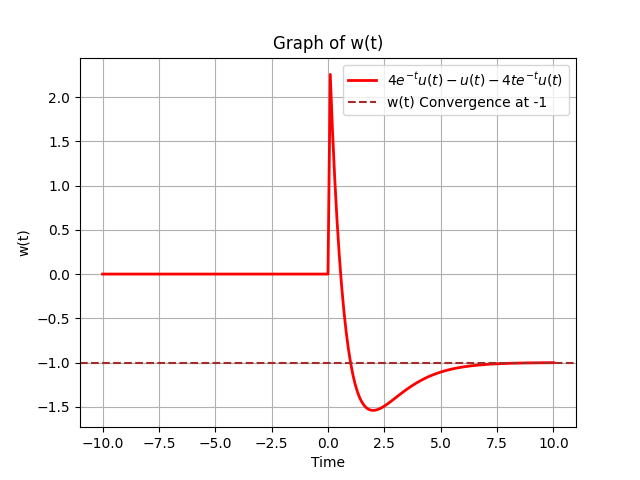
\includegraphics[width=1\columnwidth]{2023/EE/14/figs/Plot of w(t).png}
    \caption{$w\brak{t}$ converges at -1.}
    \label{fig:w_t}
\end{figure}

\begin{figure}[H]
    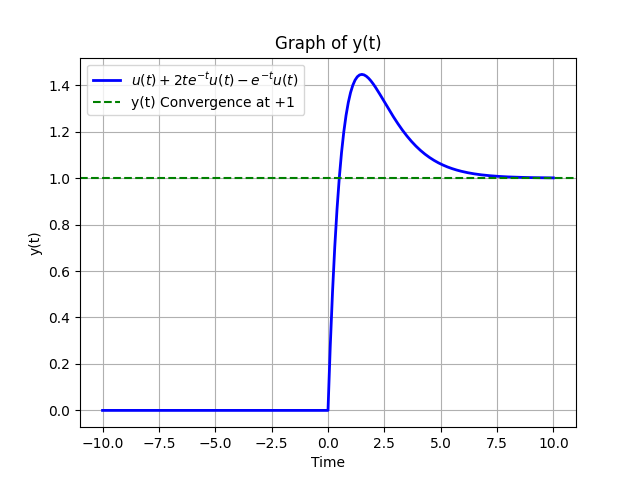
\includegraphics[width=1\columnwidth]{2023/EE/14/figs/Plot of y(t).png}
    \caption{$y\brak{t}$ converges at +1}
    \label{fig:y_t}
\end{figure}

\end{enumerate}
%\end{document}


\newpage

\item Level \brak{h} in a steam boiler is controlled by manipulating the flow rate \brak{F} of the break-up(fresh) water using a proportional \brak{P} controller. The transfer function between the output and the manipulated input is   \\
$$ \frac{h\brak{s}}{F\brak{s}}=\frac{0.25\brak{1-s}}{s\brak{2s+1}} $$   \\
The measurement and the valve transfer functions are both equal to 1. A process engineer wants to tune the controller so that the closed loop response gives the decaying oscillations under the servo mode. Which one of the following is the CORRECT value of the controller gain to be used by the engineer? \\
\begin{enumerate}[label=(\alph*)]
    \item $0.25$
    \item $2$
    \item $4$
    \item $6$
\end{enumerate} \hfill{GATE CH 2023} \\

\solution
\newpage
\item \iffalse
\let\negmedspace\undefined
\let\negthickspace\undefined
\documentclass[journal,12pt,twocolumn]{IEEEtran}
\usepackage{cite}
\usepackage{amsmath,amssymb,amsfonts,amsthm}
\usepackage{algorithmic}
\usepackage{graphicx}
\usepackage{textcomp}
\usepackage{xcolor}
\usepackage{txfonts}
\usepackage{listings}
\usepackage{enumitem}
\usepackage{mathtools}
\usepackage{gensymb}
\usepackage{comment}
\usepackage[breaklinks=true]{hyperref}
\usepackage{tkz-euclide} 
\usepackage{listings}
\usepackage{gvv}                                        
\def\inputGnumericTable{}                                 
\usepackage[latin1]{inputenc}                                
\usepackage{color}                                            
\usepackage{array}                                            
\usepackage{longtable}                                       
\usepackage{calc}                                             
\usepackage{multirow}                                         
\usepackage{hhline}                                           
\usepackage{ifthen}                                           
\usepackage{lscape}
\usepackage{placeins}
\usepackage{xparse}


\newtheorem{theorem}{Theorem}[section]
\newtheorem{problem}{Problem}
\newtheorem{proposition}{Proposition}[section]
\newtheorem{lemma}{Lemma}[section]
\newtheorem{corollary}[theorem]{Corollary}
\newtheorem{example}{Example}[section]
\newtheorem{definition}[problem]{Definition}
\newcommand{\BEQA}{\begin{eqnarray}}
\newcommand{\EEQA}{\end{eqnarray}}
\newcommand{\define}{\stackrel{\triangle}{=}}
\theoremstyle{remark}
\newtheorem{rem}{Remark}

\graphicspath{ {./figs/} } 

\begin{document}

\bibliographystyle{IEEEtran}
\vspace{3cm}

\Large\title{GATE ME 30}
\large\author{EE23BTECH11032 - Kaustubh Parag Khachane $^{*}$% <-this % stops a space
}
\maketitle
\newpage
\bigskip

\renewcommand{\thefigure}{\theenumi}
\renewcommand{\thetable}{\theenumi}
\large\textbf{Question GATE ME 30} :\\
The figure shows a block of mass m = 20 kg attached to a pair of identical linear springs, each having a spring constant k = 1000 N/m. The block oscillates on a frictionless horizontal surface. Assuming free vibrations, the time taken by the block to complete ten oscillations is \rule{1cm}{0.15mm} seconds . (Rounded off to two decimal places) Take $\pi$ = 3.14. \\ \hfill(GATE ME 2023)

\begin{figure}[!ht]
\centering
\begin{center}
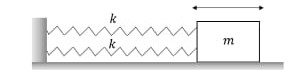
\includegraphics[width=\columnwidth]{2023/ME/30/figs/questiondiagram.jpg}
\end{center}
%\caption{Diagram for GATE ME Question 30}
\end{figure}

\solution\\
\fi
\begin{table}[!ht] 
\centering
\setlength{\extrarowheight}{8pt}
\begin{tabular}{|l|l|l|}
    \hline
    \textbf{Parameter} & \textbf{Description} & \textbf{Value} \\
    \hline
     $k_i$ & spring constant & 1000 N/m \\
    \hline
     m & mass of block & 20Kg \\
    \hline
    k & Equivalent spring constant& $k_1 + k_2$ (parallel)\\
    \hline
     $\omega_n$ & Natural frequency & $\sqrt{\frac{k}{m}}$ \\
    \hline
    T & Time period of an oscillation & $\frac{2\pi}{\omega_n}$ \\
    \hline
    x & Displacement of block & \\
    \hline
    a & Acceleration of block & $\frac{d^2x}{dt^2}$\\
    \hline
    F & Force on block & \\
    \hline
    A & Amplitude of oscillation & x\brak{0}\\
    \hline
  \end{tabular}
  \vspace{4mm}
 \caption{Parameter Table}
 \label{tab:table0_me30_2023}
\end{table}

\begin{align}
    F &= ma \\
    F &= -kx \\
    \implies ma + kx &= 0\\
    \therefore m\frac{d^2x}{dt^2} + kx &= 0\label{eq:eq1_me30_2023}
\end{align}
The Laplace transform of the terms is ,
\begin{align}
    x & \system{\mathcal{L}} X\brak{s}\label{eq:eq3_me30_2023}\\
    \frac{d^2x}{dt^2} & \system{\mathcal{L}} s^2 X\brak{s} - sx\brak{0} - \dot{x}\brak{0}\label{eq:eq2_me30_2023}
\end{align}
Using equation \eqref{eq:eq3_me30_2023} and \eqref{eq:eq2_me30_2023} in equation \eqref{eq:eq1_me30_2023},
\begin{align}
    &m\brak{s^2 X\brak{s} - sx\brak{0} - \dot{x}\brak{0}} + kX\brak{s} = 0\\
    &ms^2X\brak{s} -msA + kX\brak{s} = 0
\end{align}
\begin{align}
    X\brak{s} &= \frac{msA}{ms^2 + k} \\
     &= \frac{sA}{s^2 + \frac{k}{m}} \label{eq:eq4_me30_2023}
\end{align}
The inverse Laplace transform of such terms is given by,
\begin{align}
    \frac{s}{s^2 + a^2} \system{\mathcal{L^{ -}}} cos\brak{at}u\brak{t}
\end{align}
$\therefore$ the inverse Laplace of \eqref{eq:eq4_me30_2023} is,
\begin{align}
    x\brak{t} = Acos\brak{\sqrt{\frac{k}{m}}t} \label{eq:eq5_me30_2023}
\end{align}
From equation \eqref{eq:eq5_me30_2023} and \tabref{tab:table0_me30_2023} ,the time to complete one oscillation is,
\begin{align}
    T_n &= \frac{2\pi}{\sqrt{\frac{k}{m}}}\\
    &= \frac{\pi}{5}\label{eq:eq6_me30_2023}
\end{align}
$\therefore$ the time required for 10 oscillations is ,
\begin{align}
    10T_n &= 2\pi\\
    &= 6.28 s
\end{align}
\begin{figure}[!ht]
\centering
\begin{center}
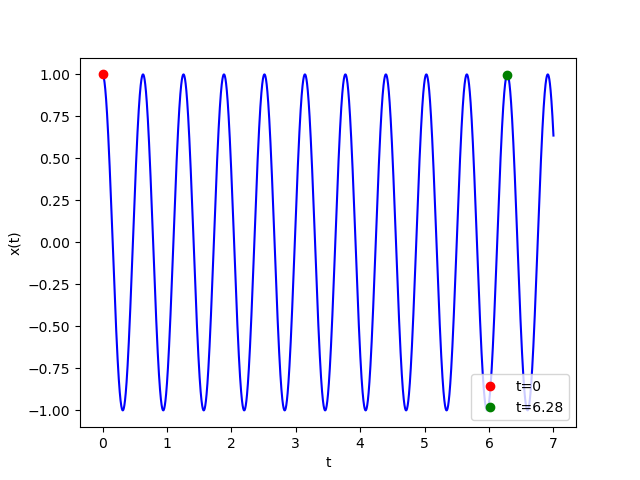
\includegraphics[width=\columnwidth]{2023/ME/30/figs/Figure_1.png}
\end{center}
\caption{Plot of $x\brak{t}$}
\end{figure}


\item A system has transfer function
 \[\frac{Y(s)}{X(s)}=\frac {s-\pi}{s+\pi}\]
 let $u(t)$ be the unit step function.The input $x(t)$ that results in a steady-state output $y(t)=sin(\pi t)$ is \underline{\quad}.\hfill (GATE IN 2023)\\
 \solution
 \newpage
 \item The state equation of a second order system is \\
$ \dot{\bm{x}}(t) = A\bm{x}(t)$, \quad $\bm{x}(0)$ is the initial condition. \\
Suppose $\lambda_1$ and $\lambda_2$ are two distinct eigenvalues of $A$, and $\nu_1$ and $\nu_2$ are the corresponding eigenvectors. For constants $\alpha_1$ and $\alpha_2$, the solution, $\bm{x}(t)$, of the state equation is \\
\begin{enumerate}[label=(\Alph*)]
\item $\sum_{i=1}^{2} \alpha_ie^{\lambda_it}\bf{\nu}_i$
\item $\sum_{i=1}^{2} \alpha_ie^{2\lambda_it}\bf{\nu}_i$
\item $\sum_{i=1}^{2} \alpha_ie^{3\lambda_it}\bf{\nu}_i$
\item $\sum_{i=1}^{2} \alpha_ie^{4\lambda_it}\bf{\nu}_i$
\end{enumerate}
\hfill{GATE 2023 EC Question 43} \\
\newpage
\item Consider the complex function
\[ f(z) = \frac{z^{2}\sin z}{(z-\pi)^4} \]
At \( z = \pi \), which of the following options is (are) correct?
\begin{enumerate}[label=\textbf{\arabic*.}, font=\bfseries, align=left]
    \item[(A)] The order of the pole is 4 
    \item[(B)] The order of the pole is 3 
    \item[(C)] The residue at the pole is \( \frac{\pi}{6} \)
    \item[(D)] The residue at the pole is \( \frac{2\pi}{3} \)
\end{enumerate}
\hfill (GATE PH 2023)
\newpage
 \item
 A buoy of virtual mass $30$ kg oscillates in a fluid medium as a single degree of
freedom system. If the total damping in the system is set as $188.5$ N-s/m, such
that the oscillation just ceases to occur, then the natural period of the system is
\rule{1cm}{0.15mm} s (round off to one decimal place)
\hfill(GATE MN 2023 question 63)\\


\item For the block diagram shown in the figure, the transfer function $\frac{Y\brak{s}}{R\brak{s}}$ is \\
\begin{figure}[H]
    {\tikzset{
    block/.style = {draw, fill=white, rectangle, minimum height=1cm, minimum width=1cm},
    plus/.style= {draw, fill=white, circle, node distance=1cm, append after command={\pgfextra \draw ($(\tikzlastnode.center) + (-0.15,0)$) -- ($(\tikzlastnode.center) + (0.15,0)$) node[above] {$+$}; \endpgfextra}},
    input/.style = {coordinate},
    output/.style = {coordinate}
}


\begin{tikzpicture}[node distance=2cm,>=latex]
    \node [input] (input) at (0,0){};
    \node [block] (block1) at (2,-2){$2$};
    \node [block] (block2) at (6,-2){$3$};
    \node [plus] (sum1) at (2,-4) {};
    \node [plus] (sum2) at (6,-4){};
    \node [block] (block3) at (4,-4) {$\frac{1}{s}$};
    \node [output] (output) at (8,-4){};
    \node [block] (block4) at (4,-6){1};
    
    \draw (input) -- node[above]{$R\brak{s}$} (2,0) to (6,0);
    \draw [->] (6,0) -- (block2);
    \draw [->] (2,0) -- (block1);
    \draw [->] (block1) -- (sum1);
    \draw [->] (sum1) -- (block3);
    \draw [->] (block3) -- (sum2);
    \draw [->] (sum2) -- node[above]{$Y\brak{s}$}(output);
    \draw [->] (block2) -- (sum2);
    \draw (7,-4) to (7,-6);
    \draw [->] (7,-6) -- (block4);
    \draw (block4) to (2,-6);
    \draw [->] (2,-6) to (sum1);  
\end{tikzpicture}
}
    \caption{Block diagram}
    \label{fig:gate_ee_Q12_blockdiagram}
\end{figure}
\hfill (GATE EE 2023)\\
\solution
\newpage

\end{enumerate}
